% Note that the a4paper option is mainly intended so that authors in
% countries using A4 can easily print to A4 and see how their papers will
% look in print - the typesetting of the document will not typically be
% affected with changes in paper size (but the bottom and side margins will).
% Use the testflow package mentioned above to verify correct handling of
% both paper sizes by the user's LaTeX system.
%
% Also note that the "draftcls" or "draftclsnofoot", not "draft", option
% should be used if it is desired that the figures are to be displayed in
% draft mode.
%
\documentclass[conference]{IEEEtran}
% Add the compsoc option for Computer Society conferences.
%

% Some very useful LaTeX packages include:
% (uncomment the ones you want to load)


% *** MISC UTILITY PACKAGES ***
%
%\usepackage{ifpdf}
% Heiko Oberdiek's ifpdf.sty is very useful if you need conditional
% compilation based on whether the output is pdf or dvi.
% usage:
% \ifpdf
%   % pdf code
% \else
%   % dvi code
% \fi
% The latest version of ifpdf.sty can be obtained from:
% http://www.ctan.org/tex-archive/macros/latex/contrib/oberdiek/
% Also, note that IEEEtran.cls V1.7 and later provides a builtin
% \ifCLASSINFOpdf conditional that works the same way.
% When switching from latex to pdflatex and vice-versa, the compiler may
% have to be run twice to clear warning/error messages.






% *** CITATION PACKAGES ***
%
\usepackage{cite}
% cite.sty was written by Donald Arseneau
% V1.6 and later of IEEEtran pre-defines the format of the cite.sty package
% \cite{} output to follow that of IEEE. Loading the cite package will
% result in citation numbers being automatically sorted and properly
% "compressed/ranged". e.g., [1], [9], [2], [7], [5], [6] without using
% cite.sty will become [1], [2], [5]--[7], [9] using cite.sty. cite.sty's
% \cite will automatically add leading space, if needed. Use cite.sty's
% noadjust option (cite.sty V3.8 and later) if you want to turn this off
% such as if a citation ever needs to be enclosed in parenthesis.
% cite.sty is already installed on most LaTeX systems. Be sure and use
% version 4.0 (2003-05-27) and later if using hyperref.sty. cite.sty does
% not currently provide for hyperlinked citations.
% The latest version can be obtained at:
% http://www.ctan.org/tex-archive/macros/latex/contrib/cite/
% The documentation is contained in the cite.sty file itself.






% *** GRAPHICS RELATED PACKAGES ***
%
\ifCLASSINFOpdf
  \usepackage[pdftex]{graphicx}
  % declare the path(s) where your graphic files are
  % \graphicspath{{../pdf/}{../jpeg/}}
  % and their extensions so you won't have to specify these with
  % every instance of \includegraphics
  % \DeclareGraphicsExtensions{.pdf,.jpeg,.png}
\else
  % or other class option (dvipsone, dvipdf, if not using dvips). graphicx
  % will default to the driver specified in the system graphics.cfg if no
  % driver is specified.
  % \usepackage[dvips]{graphicx}
  % declare the path(s) where your graphic files are
  % \graphicspath{{../eps/}}
  % and their extensions so you won't have to specify these with
  % every instance of \includegraphics
  % \DeclareGraphicsExtensions{.eps}
\fi
% graphicx was written by David Carlisle and Sebastian Rahtz. It is
% required if you want graphics, photos, etc. graphicx.sty is already
% installed on most LaTeX systems. The latest version and documentation
% can be obtained at: 
% http://www.ctan.org/tex-archive/macros/latex/required/graphics/
% Another good source of documentation is "Using Imported Graphics in
% LaTeX2e" by Keith Reckdahl which can be found at:
% http://www.ctan.org/tex-archive/info/epslatex/
%
% latex, and pdflatex in dvi mode, support graphics in encapsulated
% postscript (.eps) format. pdflatex in pdf mode supports graphics
% in .pdf, .jpeg, .png and .mps (metapost) formats. Users should ensure
% that all non-photo figures use a vector format (.eps, .pdf, .mps) and
% not a bitmapped formats (.jpeg, .png). IEEE frowns on bitmapped formats
% which can result in "jaggedy"/blurry rendering of lines and letters as
% well as large increases in file sizes.
%
% You can find documentation about the pdfTeX application at:
% http://www.tug.org/applications/pdftex



\usepackage{color}

% *** MATH PACKAGES ***
%
\usepackage[cmex10]{amsmath}
% A popular package from the American Mathematical Society that provides
% many useful and powerful commands for dealing with mathematics. If using
% it, be sure to load this package with the cmex10 option to ensure that
% only type 1 fonts will utilized at all point sizes. Without this option,
% it is possible that some math symbols, particularly those within
% footnotes, will be rendered in bitmap form which will result in a
% document that can not be IEEE Xplore compliant!
%
% Also, note that the amsmath package sets \interdisplaylinepenalty to 10000
% thus preventing page breaks from occurring within multiline equations. Use:
%\interdisplaylinepenalty=2500
% after loading amsmath to restore such page breaks as IEEEtran.cls normally
% does. amsmath.sty is already installed on most LaTeX systems. The latest
% version and documentation can be obtained at:
% http://www.ctan.org/tex-archive/macros/latex/required/amslatex/math/


% *** ALIGNMENT PACKAGES ***
%
%\usepackage{array}


% *** SUBFIGURE PACKAGES ***
\ifCLASSOPTIONcompsoc
  \usepackage[caption=false,font=normalsize,labelfont=sf,textfont=sf]{subfig}
\else
  \usepackage[caption=false,font=footnotesize]{subfig}
\fi
% subfig.sty, written by Steven Douglas Cochran, is the modern replacement
% for subfigure.sty, the latter of which is no longer maintained and is
% incompatible with some LaTeX packages including fixltx2e. However,
% subfig.sty requires and automatically loads Axel Sommerfeldt's caption.sty
% which will override IEEEtran.cls' handling of captions and this will result
% in non-IEEE style figure/table captions. To prevent this problem, be sure
% and invoke subfig.sty's "caption=false" package option (available since
% subfig.sty version 1.3, 2005/06/28) as this is will preserve IEEEtran.cls
% handling of captions.
% Note that the Computer Society format requires a larger sans serif font
% than the serif footnote size font used in traditional IEEE formatting
% and thus the need to invoke different subfig.sty package options depending
% on whether compsoc mode has been enabled.
%
% The latest version and documentation of subfig.sty can be obtained at:
% http://www.ctan.org/tex-archive/macros/latex/contrib/subfig/




% *** FLOAT PACKAGES ***
%
\usepackage{fixltx2e}
% fixltx2e, the successor to the earlier fix2col.sty, was written by
% Frank Mittelbach and David Carlisle. This package corrects a few problems
% in the LaTeX2e kernel, the most notable of which is that in current
% LaTeX2e releases, the ordering of single and double column floats is not
% guaranteed to be preserved. Thus, an unpatched LaTeX2e can allow a
% single column figure to be placed prior to an earlier double column
% figure. The latest version and documentation can be found at:
% http://www.ctan.org/tex-archive/macros/latex/base/

\usepackage{float}
\usepackage{stfloats}
% stfloats.sty was written by Sigitas Tolusis. This package gives LaTeX2e
% the ability to do double column floats at the bottom of the page as well
% as the top. (e.g., "\begin{figure*}[!b]" is not normally possible in
% LaTeX2e). It also provides a command:
%\fnbelowfloat
% to enable the placement of footnotes below bottom floats (the standard
% LaTeX2e kernel puts them above bottom floats). This is an invasive package
% which rewrites many portions of the LaTeX2e float routines. It may not work
% with other packages that modify the LaTeX2e float routines. The latest
% version and documentation can be obtained at:
% http://www.ctan.org/tex-archive/macros/latex/contrib/sttools/
% Do not use the stfloats baselinefloat ability as IEEE does not allow
% \baselineskip to stretch. Authors submitting work to the IEEE should note
% that IEEE rarely uses double column equations and that authors should try
% to avoid such use. Do not be tempted to use the cuted.sty or midfloat.sty
% packages (also by Sigitas Tolusis) as IEEE does not format its papers in
% such ways.
% Do not attempt to use stfloats with fixltx2e as they are incompatible.
% Instead, use Morten Hogholm'a dblfloatfix which combines the features
% of both fixltx2e and stfloats:
%
% \usepackage{dblfloatfix}
% The latest version can be found at:
% http://www.ctan.org/tex-archive/macros/latex/contrib/dblfloatfix/




% *** PDF, URL AND HYPERLINK PACKAGES ***
%
\usepackage{url}

% correct bad hyphenation here
\hyphenation{op-tical net-works semi-conduc-tor}


\begin{document}
\title{Experimental Framework for Testing Synchrophasor-based Damping Control Systems}


% author names and affiliations
% use a multiple column layout for up to three different
% affiliations
\author{\IEEEauthorblockN{Eldrich Rebello}
\IEEEauthorblockA{Kungliga Tekniska h\"{o}gskolan\\
Stockholm, Sweden\\
Email: rebello@kth.se}
\thanks{And so on}
\and
\IEEEauthorblockN{Luigi Vanfretti}
\IEEEauthorblockA{Kungliga Tekniska h\"{o}gskolan \\
Stockholm, Sweden \& Statnett SF, Oslo, Norway\\
Email: luigi.vanfretti@statnett.no}
\and
\IEEEauthorblockN{Md. Shoaib Almas}
\IEEEauthorblockA{Kungliga Tekniska h\"{o}gskolan\\
Stockholm, Sweden\\
Email: msalmas@kth.se}
}

% make the title area
\maketitle
%\vspace{-2em}
% As a general rule, do not put math, special symbols or citations
% in the abstract
\begin{abstract}
Wide-Area Power Oscillation Damping (WAPOD) controllers using IEEE C37.118 data have been proposed, developed and deployed in the field and are showing promise. This paper details the development, construction and implementation of a real-time, Hardware-in-the-loop (HIL) test set-up for such a controller. The set-up is based around the e\textsc{megasim} real-time simulator from OPAL-RT. A general purpose, phasor-based control algorithm is implemented on a Compact Reconfigurable Input/Output (cRIO) controller from National Instruments. The complete, closed-loop set-up, the hardware used and the reasons for design choices are also documented. Since this test-set-up uses IEEE C37.118 data over a TCP/IP network, the complete data path is examined. A test-case HIL test with the designed controller is also presented and the results are examined.

\end{abstract}

% no keywords

% For peer review papers, you can put extra information on the cover
% page as needed:
% \ifCLASSOPTIONpeerreview
% \begin{center} \bfseries EDICS Category: 3-BBND \end{center}
% \fi
%
% For peerreview papers, this IEEEtran command inserts a page break and
% creates the second title. It will be ignored for other modes.
\IEEEpeerreviewmaketitle

\section{Introduction}
\subsection{Motivation}
Instances such as the Northeast blackout of August 2003 and the August 1996 Western North America (WECC)\cite{NAERC} blackout have been significant events on large, interconnected power systems. Both can be attributed, in part, to low frequency, electromechanically induced, inter-area oscillations\cite{NAERC}. These oscillations involve the generators of one synchronous area oscillating against the generators of another area and are typically between 0.1-2Hz in frequency. The fact that these modes are poorly damped\cite{WAPODNorway} presents a danger to power systems with interconnections used for purposes such as power trading. Inter-area oscillations are also a threat to the stability of grids with significant generation coming from renewable energy sources.
%The growth of power system interconnections between previously unconnected areas has given rise to the phenomenon of inter-area oscillations. These are low frequency (0.1-2 Hz.) oscillations where the generators of one synchronous area oscillate against those of another area. Damping for these oscillations is generally poor and if they are allowed to grow, they can lead to disconnection of the ties or a collapse of the power system. A famous example of the latter was the August 1996 blackout of the WSCC system in the USA \cite{NAERC}. Although the purpose of system interconnection was to increase stability, the present situation of the power system incorporates renewable energy sources and power trading corridors, both of which impact system stability.

\subsection{Previous Experiences}
The phenomenon of intra-area oscillations is well documented and has modern solutions such as Power System Stabilisers (PSS) exist and are in use. A PSS uses locally available signals and might not be very effective at damping inter-area modes with poor local observability \cite{Yuwa}\cite{localREMcomparison}. Wide-area control systems as implemented in Norway \cite{WAPODNorway} and China \cite{WAPODChina} have extended the control system of an existing device to receive and use synchrophasor (IEEE C37.118) data.
%Modern solutions to the problem of inter-area oscillations involve using Power System Stabilisers (PSS) with locally available signals. These are effective at damping intra-area modes with good observability but may not be as effective at damping inter-area modes \cite{WAPODNorway} \cite{localREMcomparison}. Although initial field tests in \cite{WAPODNorway} \& \cite{WAPODChina} show promising results, the wide-area control systems tested so far have been implemented by extending the installed control system of an existing device (e.g. an SVC, see \cite{WAPODNorway}) to receive synchrophasor data, process it and to then feed the control algorithm. To the knowledge of the authors, there has not been any reported attempt at designing a general purpose, wire-area control system, starting from specifications and considering different hardware and software constraints. Such an approach is attractive as it can easily be adapted to different controllable elements thereby reducing implementation costs and facilitating straightforward development.
%\vspace{-0.7em}
\subsection{Contributions}
The goal of this paper is to document the details of the design and construction of a real-time test set-up for a wide-area control system. \"{A}ngquist and Gama's\cite{PhasorPOD} Phasor Power Oscillation (Phasor POD) algorithm was implemented on a Compact Reconfigurable Input-Output controller (cRIO) \cite{cRIO9081} from National Instruments which is then tested with a inputs from a two-area model\cite{KundurTwoArea} running in real-time. The entire physical test set-up is examined together with constraints of the present implementation. The results from one HIL experiment are also presented. This setup can serve as a starting point for future HIL tests that involve real-time, synchrophasor-based controllers.

\subsection*{Note}
The term 'real-time' as used in this work is identical to the sense as used in the field of embedded control\cite{Real-Time}. Though the power network used here is a simulation, it is run in real-time so any external controller based on inputs from this system would behave in an identical manner when the same inputs are sourced from an actual power network. The clock on both the real-time simulator and on the cRIO controller run as fast as an actual clock. The controller
designed is thus able to provide feedback control to the power network so as to affect the network at that point in time. Real-time is used to mean that control output generated on the controller is guaranteed to be produced in a fixed time frame. The timing limitations imposed are strict and if any delays occur, the controller is deemed to have failed. 

%\"{A}ngquist and Gama's\cite{PhasorPOD} Phasor Power Oscillation (Phasor POD) algorithm was chosen based on the operational requirements and control system design constraints. The developed prototype is termed a Wide Area Power Oscillation Damper (WAPOD). For purposes of comparison, the real-time \textsc{Simulink} implementation of the Phasor POD algorithm by Almas and Vanfretti \cite{PhasorPODImplement} is used as a benchmark. The performance of the hardware prototype developed will be tested and compared to the performance of this implementation of the algorithm. The two-area four-machine model developed by Klein, Rogers and Kundur \cite{KundurTwoArea} is used as a test-case and is modified to fit the requirements of experimental testing. A Hardware-in-the-loop experiment is constructed around the e\textsc{MEGASIM} real-time simulator from OPAL-RT \cite{OPALemegasim} with the two-area model running in real-time, physical PMUs and a synchrophasor-based Phasor-POD algorithm running on a cRIO (Figure \ref{Data_path}).


%\begin{figure}[H]
%\centering
%\includegraphics[width=3.5in]{RevisionFlow.png} 
%\vspace{-0.5em}
%\caption{General Iterative Revision Flow Diagram}
%\label{fig:RevisionFlow}
%\end{figure}


\subsection{Paper Outline}
This paper is organised as follows. Section \ref{background} outlines the damping algorithm selected, the controller architecture and introduces the two-area model used. Section \ref{hardware} presents details of the hardware used in the construction of the HIL test. Section \ref{Design} presents the design choices behind the selection of the hardware used. The HIL test and one result from it is presented in Section \ref{HILtest} and conclusions are drawn in Section~\ref{conclusion}.

\section{Background}\label{background}

\begin{figure}[!h]
\centering
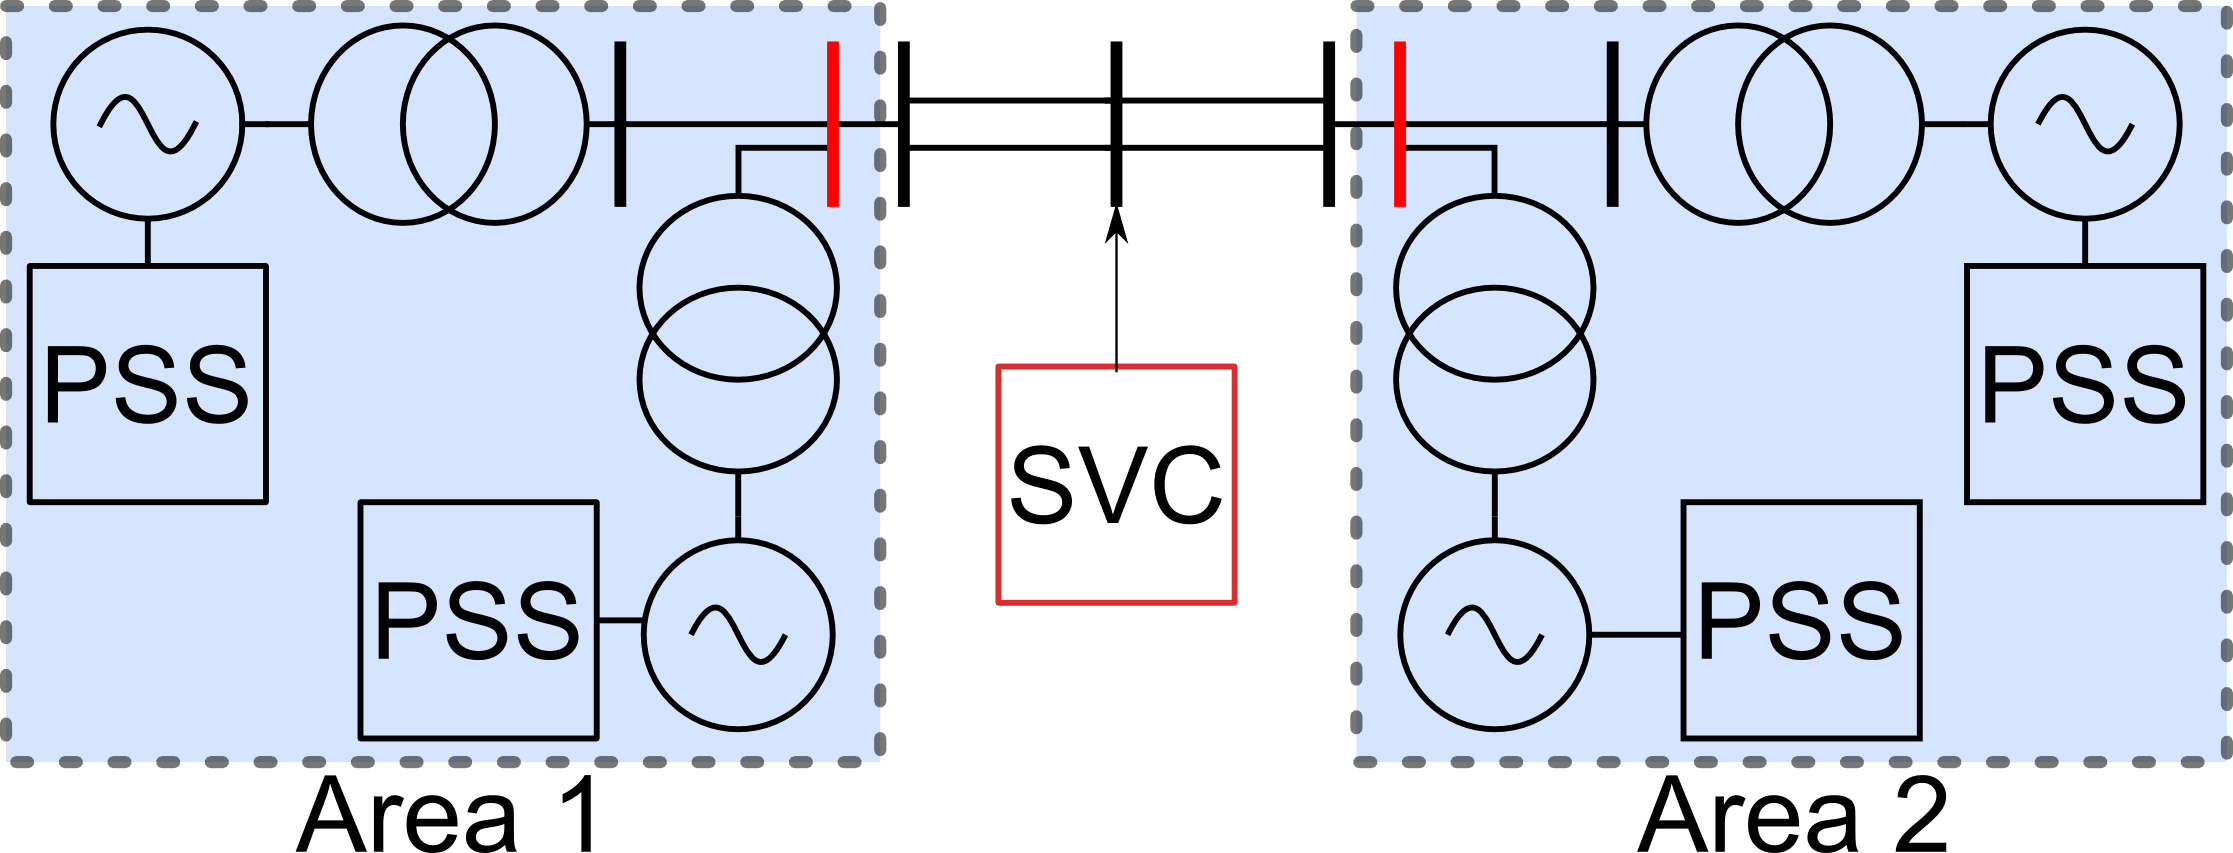
\includegraphics[width=3.5in]{TwoArea.png} 
\caption{Two-area model including SVC}
\label{TwoArea}
\end{figure}

\subsection{Two-Area Model \& Phasor POD}
The Phasor-POD algorithm essentially separates an input signal into average-valued and oscillating components \cite{PhasorPOD}. The oscillating component, when suitably phase-shifted can act as a damping input to a controllable device. This algorithm\cite{PhasorPOD} was selected due to its wide applicability and because it does not depend on network topology which can change in several situations. Typical model-linearisation based damping algorithms rely on computer-intensive calculations and are often valid for a particular network operating point and are hence not suitable for real-time implementation. In contrast, the Phasor-POD algorithm only requires knowledge of the inter-area oscillation frequency, which is generally known from system studies or can be determined from synchrophasor measurements \cite{TaskForce}. This algorithm has been demonstrated to work with a two-area model (see Figure \ref{TwoArea}) where it acts as a modulating input to a flexible AC transmission system (FACTS) device \cite{PhasorPODImplement}. The \textsc{Simulink} implementation of the Phasor-POD algorithm as presented in \cite{PhasorPODImplement} was re-written in LabView and deployed on a cRIO9081.

\subsection{Controller Architecture}
Figure \ref{FinalArch} details the three-layer controller architecture as implemented. The two-area model runs in real-time on the OPAL-RT simulator. Phasor Measurement Units (PMUs) are connected to the analogue outputs of the real-time simulator. The synchrophasor data stream that these PMUs generate is parsed on a desktop computer (Label 1 in Figure \ref{FinalArch}). This data is then sent over a TCP/IP network to the cRIO running the control algorithm. The Phasor-POD algorithm is implemented on the cRIO's FPGA which generates an analogue damping signal.

\begin{figure}[]
\centering
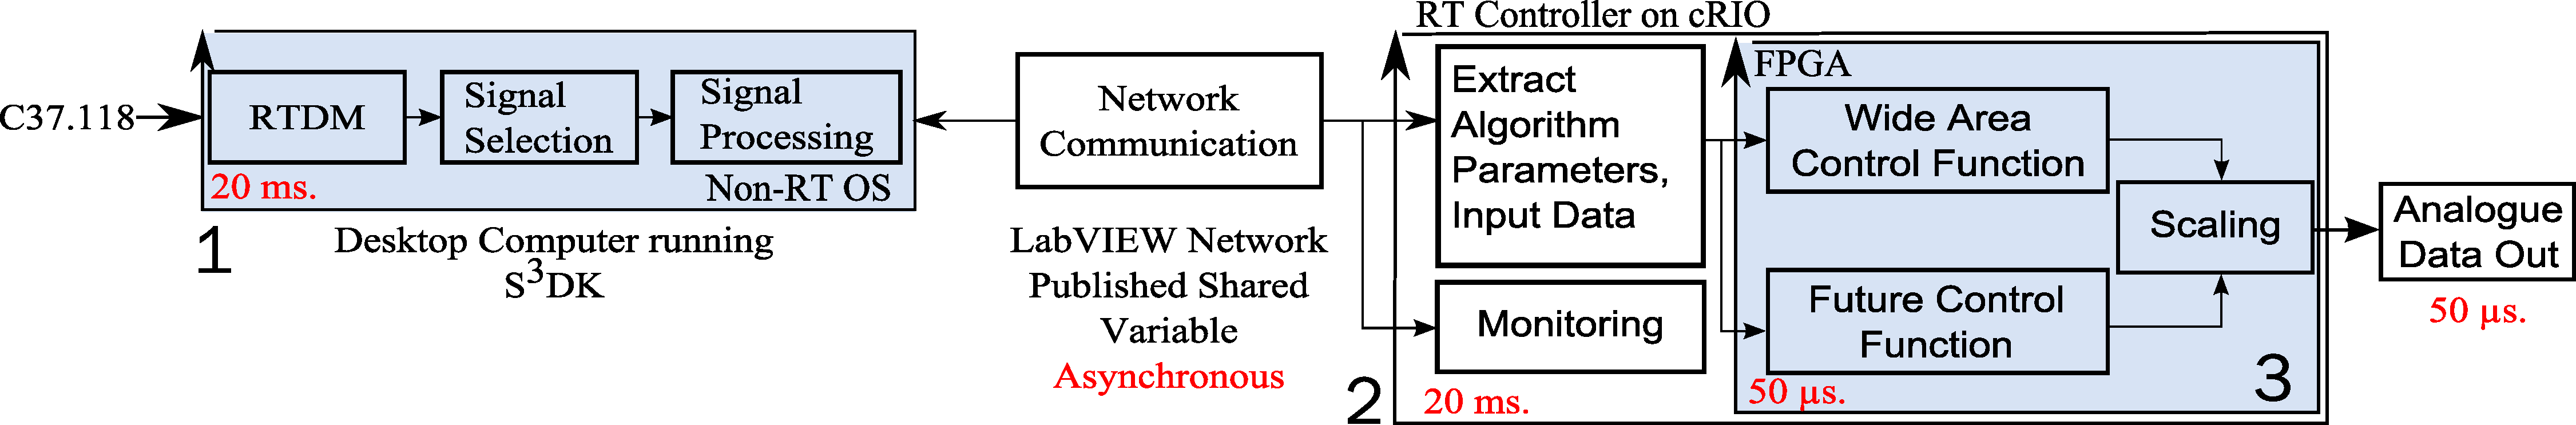
\includegraphics[width=3.5in]{ArchitectureDevelopment.pdf} 
\caption{Three layer controller architecture as implemented}
\label{FinalArch}
\end{figure}

\subsection{SmarTS Lab}
All the hardware and software detailed in this work is available in the SmarTS Lab at KTH, Stockholm. For full details of the lab, all its equipment and capabilities, the reader is referred to \cite{SmarTSLab}. This work only presents the hardware that form part of the HIL test described here and only touches upon their capabilities.

\section{Hardware \& Test Setup}\label{hardware}

Figure \ref{ExperimentOutline} presents the data path and a simplified outline of the entire HIL test conducted. This setup was arrived at after several changes to the design necessitated by limitations of the hardware and software. These are covered in the next section.

\subsection{OPAL-RT Simulator}
The e\textsc{megasim}\cite{eMEGASIM} real-time simulator from OPAL-RT\cite{OPALemegasim} was the core of the HIL test. The simulator ran the two-area \textsc{Simulink} model in real-time and allowed for interfacing hardware with the model through its analogue input and output terminals.  Details of these terminals are below.

\begin{itemize}
\item \textbf{Analogue Outputs} : Number: 32 (+/-16V and +/-10mA)
\item \textbf{Analogue Inputs} : Number: 128 (+/-100V and +/-10mA)
\end{itemize}

The simulator would calculate and update values for all variables in the two-area model every 50$\mu$s. This time step was selected to allow for the assumption of linearity of power system parameters. Updated values would be written to the analogue outputs and input values read at the analogue inputs every 50$\mu$s. The \textsc{Simulink} model was developed and edited on a workstation computer and the same computer was used to monitor output from the simulator while the model was running.

\subsection{cRIO Real-Time Controllers}
\begin{figure}[H]
\centering
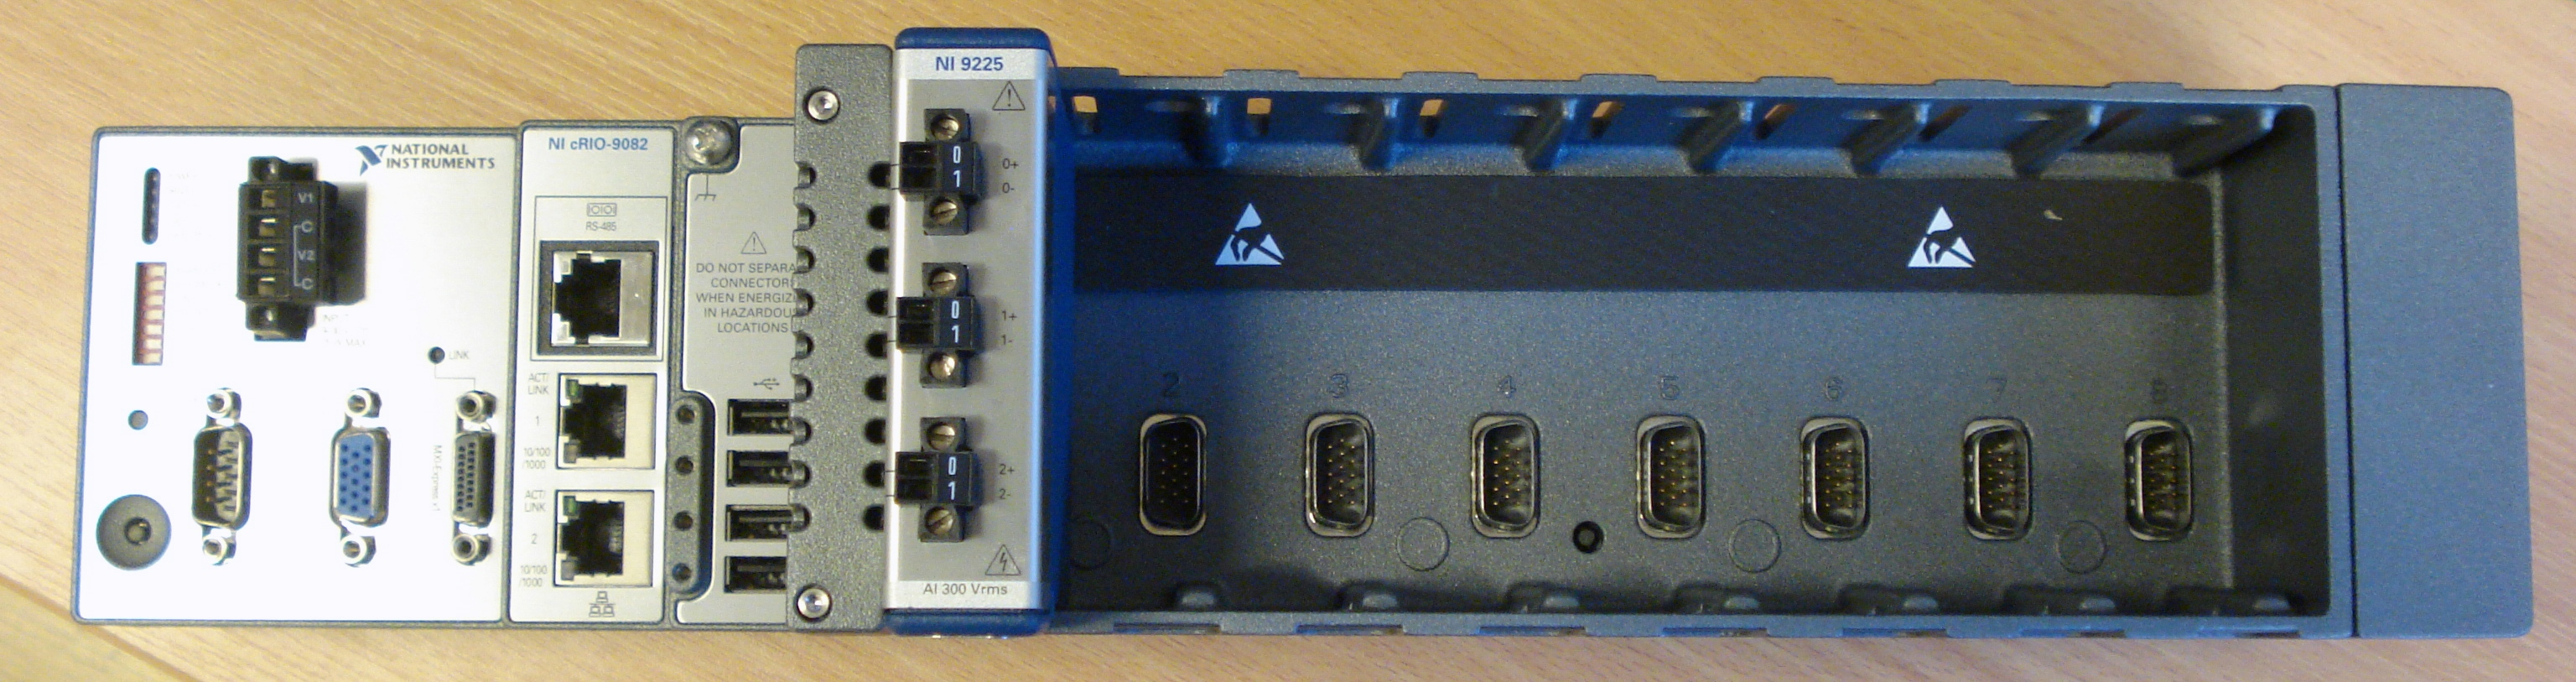
\includegraphics[width=3.5in]{DSC05446.JPG}
\vspace{-0.5em}
\caption{cRIO9081 showing NI9225, three-channel, analogue voltage input module and seven empty add-on module slots}
\label{cRIO}
\end{figure}
Two different cRIO models were used in this particular HIL test. One model, the cRIO9081, was used to run the Phasor-POD algorithm in real-time. Two cRIO9076s were deployed as PMUs. Figure~\ref{cRIO} shows the cRIO9081 with an analogue voltage input add-on module connected. The data generated by the Phasor-POD algorithm was sent as an analogue signal back to the real-time simulator. 

\subsubsection*{PMUs} Two cRIO9076s were used as PMUs, each with a four-channel, analogue voltage input module and a three-channel, analogue current input module. The inputs to the PMUs were three-phase currents and voltages and a GPS signal for time-sync. PMU software from National Instruments was run on both. The synchrophasor stream from each PMU was sent to a Phasor Data Concentrator (PDC). Each generated a C37.118 synchrophasor data stream which was sent over a TCP/IP network. The reporting rate of the PMUs was 20ms meaning that new measurements were available every 20ms. Though it was possible to generate synchrophasor data from the real-time simulator, the option of using analogue signals was chosen as it mimicked a real-world scenario. The module ratings were 0-300V and 0-5A with 24 bit resolution each\cite{cRIO9081} for the NI9225 and NI9227 respectively. To reduce subsequent computation, the PMUs were configured to compute and report values of active power.

\subsubsection*{Real-Time Phasor-POD Algorithm} The FPGA of a cRIO9081 was used to run the Phasor-POD algorithm in real-time. Though the cRIO9081 has a real-time controller in addition to the FPGA, the latter was chosen to run the Phasor-POD algorithm. This was because the FPGA runs at 400Mhz and is thus capable of a deterministic response time in the order of nanoseconds. The loop rate chosen was 50$\mu$s so that the data output rate of the FPGA was identical to the read rate on the real-time simulator's input.

\subsection{Analogue Signal Amplifiers}
The SMRT1 Single Phase Relay Tester \cite{Megger} from Megger was used as an analogue signal amplifier. Each individual amplifier had a single current and single voltage input. To drive the inputs of two PMUs, six amplifier units were required. The inputs to the amplifiers were the low-level analogue signals extracted from the real-time simulator. The outputs of the amplifiers were wired to the analogue input modules of the PMUs. Table \ref{AmplifierTable} lists the ratios used. To avoid saturation in the amplifiers, the outputs from the real-time simulator were limited to $\pm$10V. 

\begin{table}[!ht]
\caption{Amplifier Inputs and Outputs}\label{AmplifierTable}
\begin{center}
\begin{tabular}{|l|c|c|}
\hline \textbf{} & \textbf{Input, from simulator} & \textbf{Amplified Output} \\
\hline Voltage &$\pm10V$&$\pm 100V$\\ 
\hline Current & $\pm 20mA$ & $\pm 1A$\\ 
\hline 
\end{tabular}
\end{center}
\end{table} 

\subsection{Phasor Data Concentrator}
The Phasor Data Concentrator (PDC) consisted of a network connected desktop computer running PDC software from SEL. The PDC was used to allow for data from multiple synchrophasor streams to be manipulated and used. It also had data logging functionality which was used to analyse the system performance.

\begin{figure*}[!th]
\centering
%\label{ExperimentOutline}
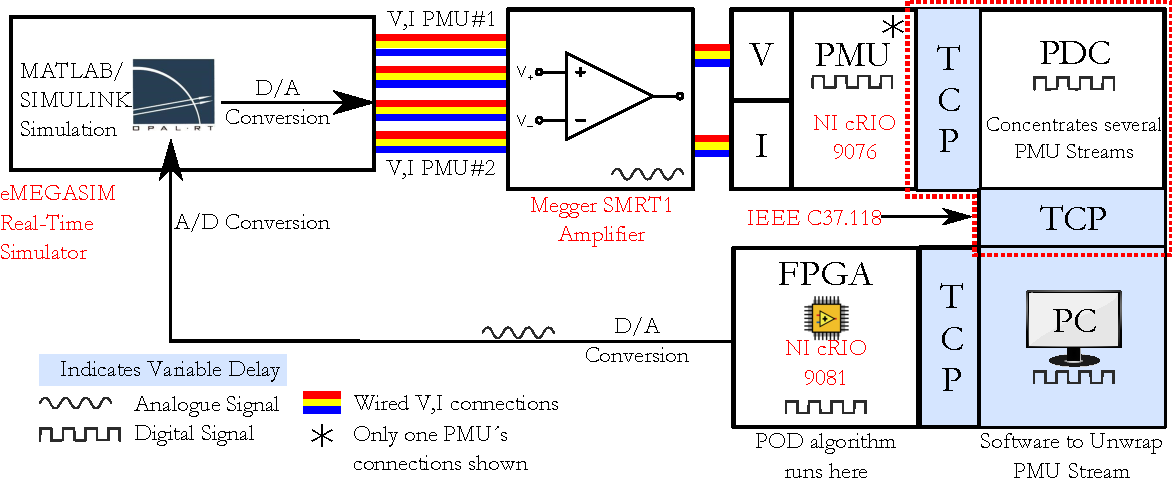
\includegraphics[width=6in]{DelaySources.pdf} 
\caption{Data path and experiment outling of HIL test. Hardware used is indicated in {\color{red}red} text. Note that two PMUs are use though one is indicated. Section where synchrophasor data is used is indicated with dotted outline.}
\label{ExperimentOutline}
\end{figure*}

\section{Hardware Design Choices} \label{Design}
Figure \ref{ExperimentOutline} shows the final HIL test setup which was used to evaluate the performance of the real-time Phasor-POD algorithm. This design was arrived at after numerous changes to the setup. This section outlines the most significant changes made together with their reasons.

\subsection{Analogue Signal Amplifiers} The initial setup envisaged connecting the analogue outputs of the real-time simulator directly to the inputs of the PMUs. This approach simplified wiring but had to be abandoned due to a poor signal-to-noise ratio. The main reason for this poor signal-to-noise ratio was the fact that a very small portion of the dynamic range of the PMU's input modules was being used. A 0-10V signal was being read by a voltage module rated for 0-300V and a 0-20mA signal was being read by a module rated for 0-5A. This resulted in the POD algorithm producing a large error signal even at steady state. Using an amplified signal as a PMU input greatly improved the signal-to-noise ratio and thus the performance of the Phasor-POD algorithm. Though the amplifiers greatly improved the signal-to-noise ratio, additional scaling factors were introduced in the simulation and in the PMUs. For instance, the analogue output of the real-time simulator had to be limited in magnitude to avoid problems such as amplifier saturation. Also, CT and PT ratios in the PMUs were used to account for scaling factors in other sections of the HIL test.

\subsection{FPGA} The Phasor-POD algorithm was implemented on the FPGA of the cRIO9081. This was despite the challenges of writing FPGA code and despite the fact that the algorithm could have been run on the real-time section of the controller. Two reasons were behind this choice. One was that the real-time section of the cRIO9081 handles asynchronous TCP/IP communication. This had to be incorporated in to a deterministic control loop which would also run the control algorithm. Any delays in the network would result in a delay in output from the control loop which would affect performance. The second problem was that the fastest loop rate that the real-time controller was capable of was 1ms. This was achievable only in ideal conditions. The real-time simulator expected input from the controller every 50$\mu$s, a rate that the real-time controller could not match. By leaving the task of network communication to the real-time controller, the FPGA was used to run the control algorithm together with a sample-and-hold algorithm and produce output every 50$\mu$s.

\subsection{Desktop Computer} An ideal controller would be able to parse the synchrophasor stream, extract measurement data and perform control action autonomously. However, no software was available that could run on the cRIO and parse the synchrophasor stream. Software \cite{SDK} was, however, available that could perform this function on a desktop computer. The solution implemented here thus has a desktop computer running a multi-tasking operating system to extract data from the synchrophasor stream. This data is then sent to the cRIO over the TCP network. In the scenario where data from multiple PMUs is used, computations such as the voltage phase angle difference are performed on this computer.

\section{Hardware-in-the-Loop Test} \label{HILtest}

A setup identical to that outlined in Figure \ref{ExperimentOutline} was constructed and used to verify the working of the hardware WAPOD. As opposed to a simulation, a HIL test has sources of delay and noise. Sources of stochastic delay are indicated in red in Figure \ref{ExperimentOutline}. Signals are extracted from the edges of Area 1 and Area 2 as indicated in Figure \ref{TwoArea} and are sent to two PMUs via analogue amplifiers. The PMUs generate a sychophasor data stream which is sent to a PDC over a TCP network. The PDC time aligns both streams and retransmits them over the same TCP network. The streams are received on a desktop computer running LabView. Here, measurement data is extracted from the streams and is sent to the control algorithm running on the cRIO. The cRIO recieves this data and passes it to the built-in FPGA which runs the Phasor-POD algorithm. The FPGA uses an analogue voltage output module to generate a control signal which is wired back to the real-time simulator. After scaling, this signal is reintroduced in the \textsc{Simulink} model running in real-time.\\
\begin{figure}[!h]
%\centering
%\label{ExperimentOutline}
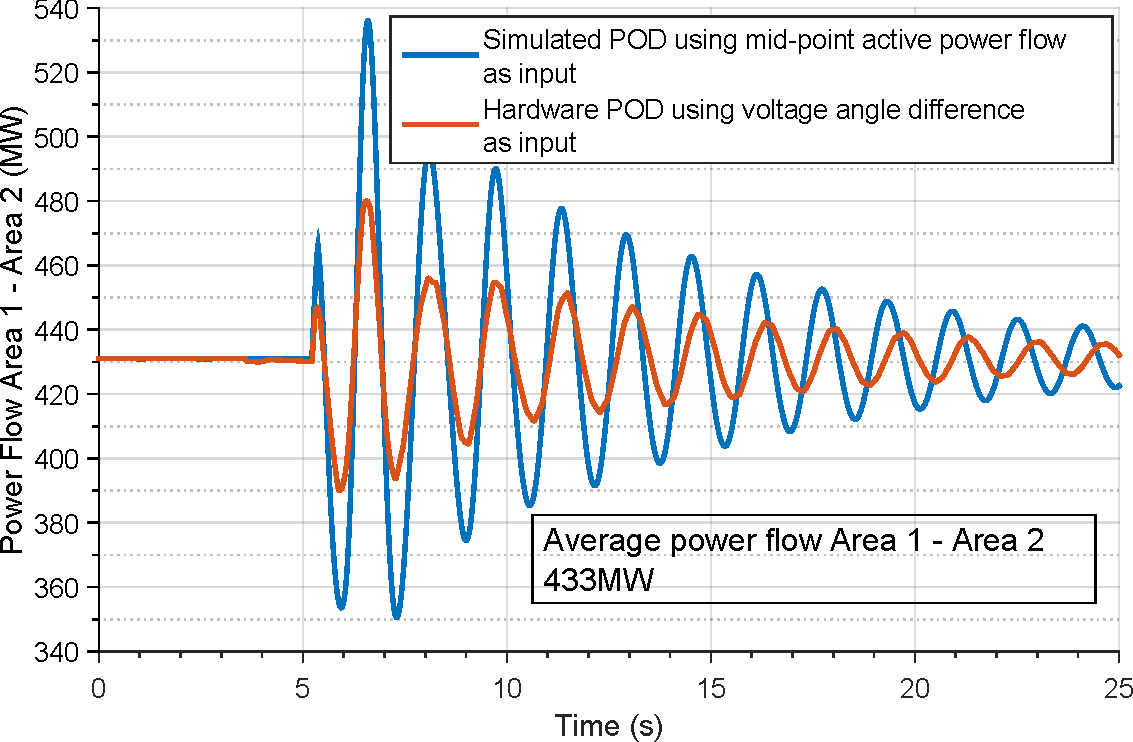
\includegraphics[width=3.5in]{SVC_ResponseComparison_Labelled.pdf} 
\caption{Output (in V) from cRIO running Phasor-POD algorithm, shown in green. Only SVC provides damping action in this case. Black plot indicates ideal response with damping from SVC at mid-point and PSS's at each mahine}
\label{HILGraph}
\end{figure}
Results from the real-time HIL test are presented in Figure~\ref{HILGraph}. The Phasor-POD algorithm running on the cRIO uses active power (outflow from Area 1) as a control input. The inter-area mode is excited at t=2s by momentarily changing the voltage reference of one generator in Area 1 before returning it to normal. As evident in Figure~\ref{HILGraph}, the Phasor-POD algorithm on the cRIO is able to restore the system to stability. As a comparison, the response of the system to the same disturbance but damped by a combination of the generator PSS and the POD (running in \textsc{Simulink}) is shown with the black plot. It is evident that the hardware implementation of the Phasor-POD algorithm is able to damp the inter-area mode and restore the system to stability. It is important to note that the black plot represents system performance with a PSS at each machine in addition to the SCV at the mid-point of the two-area network. In comparison, the green plot represents system performance with the SVC acting as the only damping element. Figure~\ref{HILGraph} is not meant to serve as a comparison but rather, confirmation, that real-time damping can be achieved with commercially available, general purpose controllers.\\

The experimental setup detailed here was designed for testing one particuar algorithm. The setup, however, is modular enough that sections of it can be replaced or removed entirely. The controller used here is based on proprietary hardware and software from National Instruments. The support, documentation and software from National Instruments greatly accelerated the development and testing of this prototype. The authors, however, would like to see similar algorithms run on open hardware platforms such as the Raspberry pi or Arduino.



\section{Conclusion} \label{conclusion}
An outline of a real-time HIL test setup used to test the Phasor-POD algorithm is presented. The hardware used in the construction of this test together with the design decisions that influenced these choices are presented. The results from one HIL experiment are presented and serve to verify the working of the real-time, hardware implementation of the Phasor-POD algorithm.
% conference papers do not normally have an appendix


% use section* for acknowledgement
\section*{Acknowledgment}
The work of E. Rebello \& M.S. Almas was supported by the STRON$g^{2}$rid project, funded by Nordic Energy Research.\\
L. Vanfretti is supported by the STRON$g^{2}$rid project, funded by Nordic Energy Research, and by the STandUP for Energy collaboration initiative and by Statnett SF, the Norwegian transmission system operator.
% trigger a \newpage just before the given reference
% number - used to balance the columns on the last page
% adjust value as needed - may need to be readjusted if
% the document is modified later
%\IEEEtriggeratref{8}
% The "triggered" command can be changed if desired:
%\IEEEtriggercmd{\enlargethispage{-5in}}
%\section*{Acknowledgment}
%\vspace{-1em}
%\begin{figure}[htb]
%\centering
%\includegraphics[width=2.5in]{Best_sample.png}
%\vspace{-0.5em}
%\caption{Controller Response with Voltage Angle Difference input captured using an Oscilloscope}
%\label{ScopeCapture}
%\end{figure}
% references section

% can use a bibliography generated by BibTeX as a .bbl file
% BibTeX documentation can be easily obtained at:
% http://www.ctan.org/tex-archive/biblio/bibtex/contrib/doc/
% The IEEEtran BibTeX style support page is at:
% http://www.michaelshell.org/tex/ieeetran/bibtex/
%\bibliographystyle{IEEEtran}
% argument is your BibTeX string definitions and bibliography database(s)
%\bibliography{IEEEabrv,../bib/paper}
%
% <OR> manually copy in the resultant .bbl file
% set second argument of \begin to the number of references
% (used to reserve space for the reference number labels box)


\begin{thebibliography}{1}

\bibitem{NAERC} North American Electric Reliability Council \emph{Review of selected 1996 Electric System Disturbances in North America,} August 2002. Available Online: \url{http://www.nerc.com/pa/rrm/ea/System\%20Disturbance\%20Reports20DL/1996SystemDisturbance.pdf}

\bibitem{WAPODNorway} K. Uhlen, L.~Vanfretti, M.M. De Oliveira, A.B. Leirbukt,V. H. Aarstrand and J. O. Gjerde \emph{Wide-Area Power Oscillation Damper implementation and testing in the Norwegian transmission network} in Power and Energy Society General Meeting, 2012 IEEE pp. 1-7

\bibitem{localREMcomparison}  M. E.~Aboul-Ela, A. A.~Sallam, J. D.~McCalley and A. A.~Fouad, \emph{Damping Controller Design for Power System Oscillations Using Global Signals}, IEEE trans. on Power Systems, Vol. 11, No. 2, May 1996, pp. 767-773

\bibitem{Yuwa}  L.~Vanfretti, Y.~Chompoobutrgool, and J.H.~Chow, \emph{Chapter 10: Inter-Area Mode Analysis for Large Power Systems using Synchrophasor Data}, Book Chapter, in Coherency and Model Reduction of Large Power Systems, Joe H. Chow (Ed.), Springer, 2013.

\bibitem{WAPODChina} Li Peng and Wu Xiaochen and Lu Chao and Shi Jinghai and Hu Jiong and He Jingbo and Zhao Yong and Aidong Xu \emph{Implementation of CSG's Wide-Area Damping Control System: Overview and experience} in Power Systems Conference and Exposition, 2009. PSCE '09. IEEE/PES pp. 1-9

\bibitem{PhasorPOD} L.~\"{A}ngquist and C.~Gama  \emph{Damping Algorithm based on Phasor Estimation} in Power Engineering Society Winter Meeting, 2001. IEEE, Volume 3, pp. 1160 - 1165  

\bibitem{TaskForce} M.Crow, M. Gibbard, A. Messina, J. Pierre, J. Sanchez-Gasca, D. Trudnowski, D. Vowles \emph{Identification of Electromechanical Modes in Power Systems} IEEE Task Force Report, Special Publication TP462, June2012.

\bibitem{Real-Time} Ben-Ari, M., "Principles of Concurrent and Distributed Programming", Prentice Hall, 1990. ISBN 0-13-711821-X. Ch16, Page 164

\bibitem{PhasorPODImplement} M.~Shoaib Almas and L.~Vanfretti, \emph{Implementation of Conventional PSS and Phasor Based POD for Power Stabilizing Controls for Real-Time Simulation}, IEEE IES IECON14, 29 Oct-1 Nov, 2014, Dallas, USA.

\bibitem{KundurTwoArea} 
M.~Klein, J. G.~Rogers and P.~Kundur \emph{A fundamental study of inter-area oscillations in Power Systems} IEEE Trans, PWRS, no. 6, pp. 914-921, 1991.

\bibitem{OPALemegasim} eMEGAsim PowerGrid Real-Time Digital Hardware in the Loop Simulator — Opal RT, [Online]. Available: \url{http://www.opal-rt.com/}

\bibitem{cRIO9081} \emph{Operating Instructions and Specifications Compact RIO NI cRIO-9075/9076 \& NI cRIO-9081/9082}, National Instruments, Available Online at \url{http://www.ni.com/}

\bibitem{PMUMario} M. Paolone, A. Borghetti, C. A. Nucci, \emph{A Synchrophasor Estimation Algorithm for the Monitoring of Active Distribution Networks in Steady State and Transient Conditions}, Proc. of the 17th Power Systems Computation Conference (PSCC 2011), Stockholm, Sweden, Aug. 22-26, 2011 

\bibitem{SIMULINKOnline} Kamwa \ I. (Hydro-Quebec) "Performance of Three PSS for Interarea Oscillations" Available Online at : \url{http://www.mathworks.se/help/physmod/sps/examples_v2/performance-of-three-pss-for-interarea-oscillations.html}

\bibitem{eMEGASIM} \emph{eMEGASIM Power Grid Real-Time Digital HArdware in the Loop Simulator} Available Online at : \url{http://www.opal-rt.com/}

%\bibitem{Dmello} F. P.~Dmello, and C.~Concordia \emph{Concepts of Synchronous Machine Stability as Affected by Excitation Control} IEEE Transactions on Power Apparatus and Systems, vol. PAS 88, no. 4, 1969. 

\bibitem{SmarTSLab} M.S. Almas, M. Baudette, L. Vanfretti, S. Lovlund and J.O. Gjerde "\emph{Synchrophasor network, laboratory and software applications developed in the STRON$g^{2}$rid project}," PES General Meeting, Conference Exposition, July 2014 IEEE pp 1 - 5

\bibitem{Megger} SMRT1 Single Phase Relay Test System Data Sheet, Available Online \url{http://www.megger.com/common/documents/SMRT1_DS_en_V10.pdf} Retreived 22.12.2014, 2014 \textcopyright~Megger

%\bibitem{Chaudhuri} N.S.~Chaudhuri, R.~Majumder and B~ Chaudhuri \emph{Interaction between conventional and adaptive phasor power oscillation damping controllers} in Power and Energy Society General Meeting, 2010 IEEE Minneapolis, MN, 2012 pp. 1-7

%\bibitem{sVARdamp} E.V~Larsen and E.H~Chow, General Electric Company, NY, \emph{SVC control design concepts for system dynamic performance}, in Application of Static Var Systems for System Dynamic Performance 1987, IEEE, pp. 36-53

%\bibitem{cRIO9076} \emph{Operating Instructions and Specifications Compact RIO NI cRIO-9075/9076}, National Instruments, Available Online at \url{http://www.ni.com/pdf/manuals/375650b.pdf}

%\bibitem{LabviewTemplate} \emph{FPGA Control on Compact RIO Sample Project Documentation}, National Instruments, Available Online at \url{http://www.ni.com/white-paper/14137/en/}

\bibitem{SDK} L. Vanfretti, V.H. Aarstrand, M. Shoaib Almas, V. S. Peri\'c and J.O Gjerde \emph{A Software Development Toolkit for Real-Time Synchrophasor Applications},  IEEE PES Grenoble PowerTech, 2013

%\bibitem{MATLABexample} I~Kamwa \emph{Performance of Three PSS for Interarea Oscillations} SimPowerSystems Examples, \textsc{Matlab} R2011a

%\bibitem{PSSDocumentation} \emph{Generic Power System Stabilizer} Documentation distributed with \textsc{Matlab} R2014a Available online at \url{http://www.mathworks.se/help/physmod/sps/powersys/ref/genericpowersystemstabilizer.html}

%\begin{figure}[]
%\centering
%\includegraphics[width=3in]{LabVIEWProj.JPG}
%\caption{LabView Project Explorer showing different sections of code and the devices on which they run. \textbf{This image is too tall to fit within the text. I wanted to include this as an appendix but the Latex file says that conference papers generally don't have appendices.
%}}
%\label{LabProject}
%\end{figure}

\end{thebibliography}
%\bibliography{references}
%\begin{figure*}[ht]
%\centering
%\includegraphics[width=6in]{LabView_Numbered}
%\caption{Outline of the SmarTS Lab. Corresponding to Numbers: 1: Real Time Simulator, 2: PDC Interface, 3: cRIO Tray, 4: Oscilloscope, 5: Analogue Signal Amplifiers, 6: SEL Protection Relays}
%\label{fig:LabView_Numbered}

\end{document}


